%Copyright (c) 2004 2005 2006 Atos Origin
%Permission is granted to copy, distribute and/or modify this
%document
%under the terms of the GNU Free Documentation License,
%      Version 1.2
%      or any later version published by the Free Software
%      Foundation;
%      with no Invariant Sections, no Front-Cover
%      Texts, and no Back-Cover
%      Texts.  A copy of the license is
%      included in the section entitled "GNU
%      Free Documentation License".
%
%$Id: define.tex,v 1.2 2006/03/07 16:35:51 rsemeteys Exp $
\section{Definition}
\begin{figure}
\center
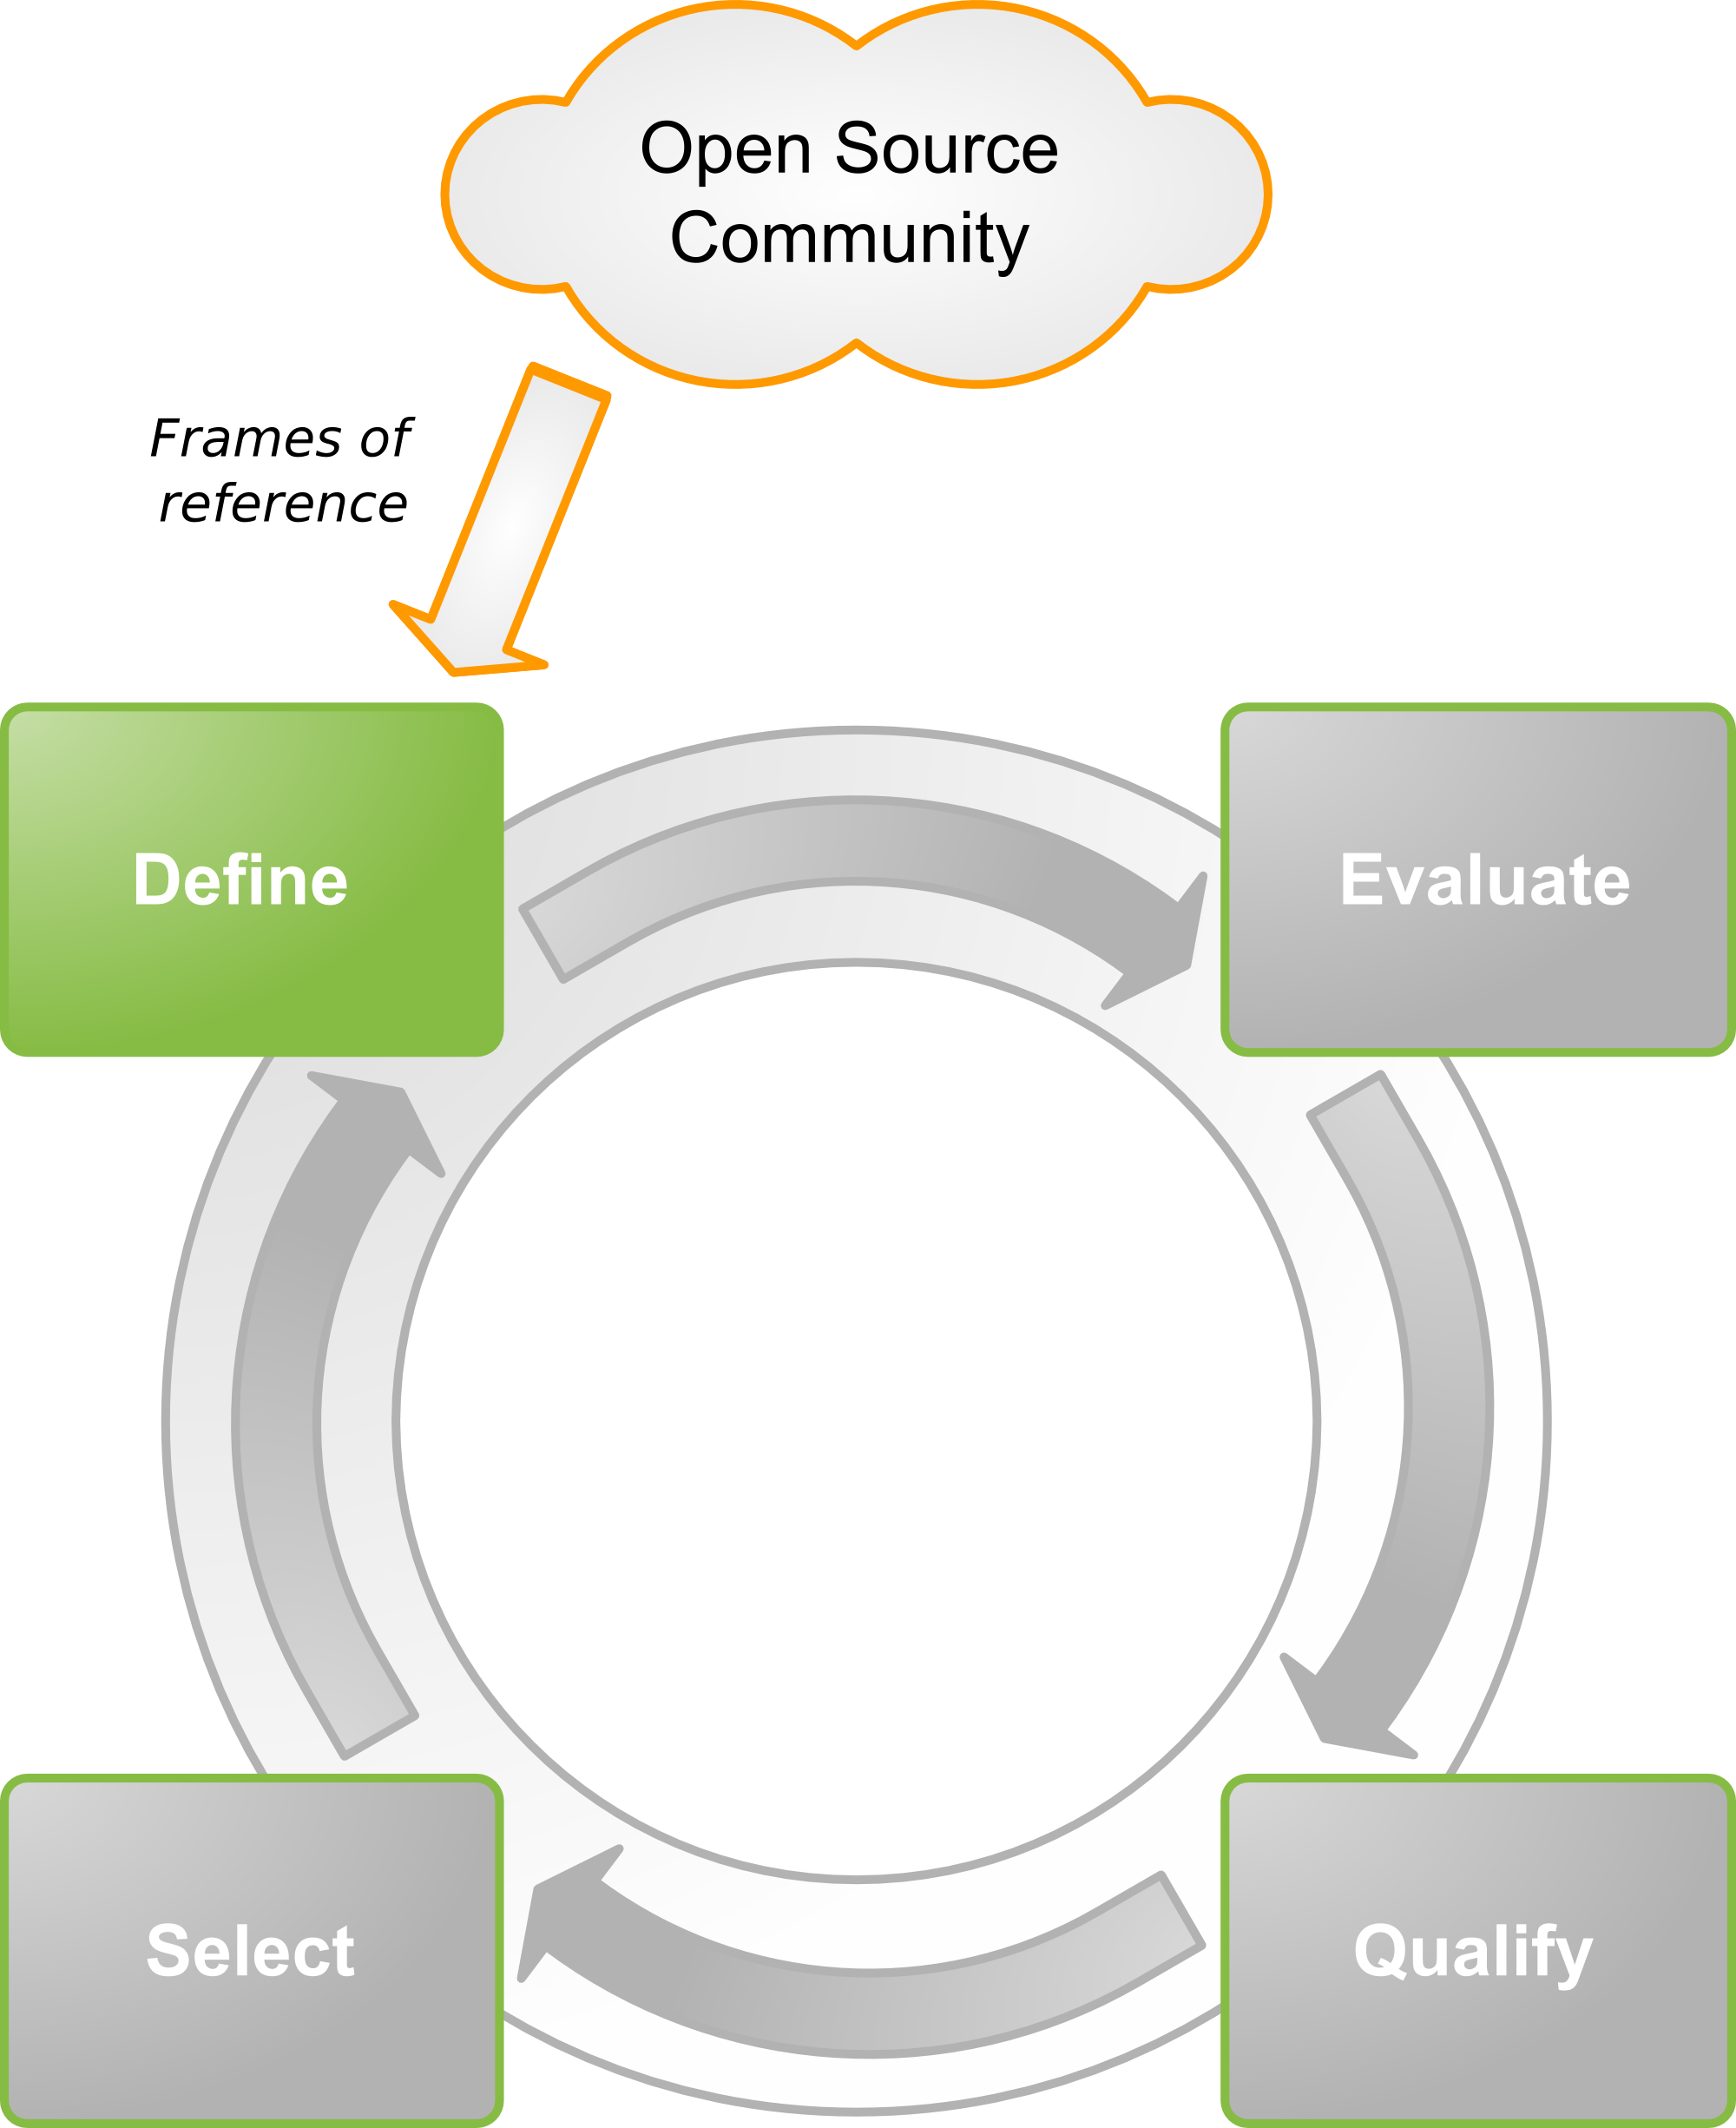
\includegraphics[width=10cm]{images/definir}
\caption{Step 1 - Definition}
\end{figure}


\subsection{Objective}
The objective of this step is to define various elements of the typology re-used by the three 
remaining steps of the general process.


The frames of reference are :
\begin{description}
\item [Software families:] hierarchical classification of software domains and description of functional grids associated with each domain.
\item [Types of licences:] classification of free and open source licenses.
\item [Types of communities:] classification of community organizations existing around a free or open source software and in charge of its life-cycle.
\end{description}


\subsection{Software families}
This frame of reference evolves the most because as software evolves, it
offers new functionalities that need to be added to the frame of reference.

\subsection{Types of licences}
This frame of reference lists and classifies the major licences used for free and open source software.
The criteria chosen to describe such a license are:

\begin{description}
\item [Ownership:] can the derived code become proprietary or must it remain free?
\item [Virality:] is another module linked to the source code inevitably affected by the same license?
\item [Inheritance:] does the derived code inherit inevitably from the license or is it possible to apply additional restrictions to it?
\end{description}

The table~\ref{license-list} lists a comparison of the most common licences showing the criteria formulated above.


\begin{figure}
\center
\begin{tabular}{|c|c|c|c|}
\hline \TS{License} & \TS{Ownership} & \TS{Virality} & \TS{Inheritance}\\
\hline GPL & No & Yes & Yes\\
\hline CeCILL & No & Yes & Yes\\
%TODO revenir sur LGPL
\hline LGPL & No & Partial & Yes\\
\hline BSD & Yes & No & No\\
\hline Artistic & Yes & No & No\\
\hline MIT & Yes & No & No\\
\hline Apache v1.1 & Yes & No & No\\
\hline Apache v2.0 & Yes & No & No\\
\hline MPL v1.1 & No & No & Yes\\
\hline Common Public License v1.1 & No & No & No\\
\hline Academic Free License v2.1 & Yes & No & No\\
\hline PHP License v3.0 & Yes & No & No\\
\hline Open Software License v2.0 & No & No & No\\
\hline Zope Public License v2.0 & Yes & No & No\\
%TODO idem
\hline Python SF License v2.0 & Yes & No & No\\
\hline
\end{tabular}
\caption{Non comprehensive list of licenses}
\label{license-list}
\end{figure}
Note that a piece of software or code can be published under the terms of several licences (including closed source).

\subsection{Types of communities}
The types of communities identified to date are:
\begin{description}
\item [Insulated developer:] the software is developed and managed by only one person.
\item [Group of developers:] several people collaborating in an informal or not industrialized way.
\item [Organization of developers:] a group of developers managing the software life-cycle in a formalized way, generally based on role assignment (developer, tester, delivery manager...) and meritocracy.
\item [Legal Entity:] a legal entity (in general non lucrative) that manages the community, generally possesses copyrights and also manages sponsorship and linked subsidies.
\item [Commercial entity:] the commercial organization employing the project's main developers who are remunerated by the sale of services or of commercial versions of the software.
\end{description}


\subsection{O3S tool}
The O3S tool is designed to be able to easily manage these frames of reference and to measure 
impacts generated by modifications on data already collected during others QSOS steps.
